%%%%%%%%%%%%%%%%%%%%%%%%%%%%%%%%%%%%%%%%%%%%%%%%%%%%%%%%%%%%%%%%%%%%%%
% Introduction to Quantum Computing
%%%%%%%%%%%%%%%%%%%%%%%%%%%%%%%%%%%%%%%%%%%%%%%%%%%%%%%%%%%%%%%%%%%%%%

\documentclass[11pt,a4paper]{report}

%-------------------------
% Package Imports
%-------------------------
\usepackage{amsmath,amssymb,amsfonts,amsthm}
\usepackage{mathtools,commath}
\usepackage{bm}            % for bold math symbols

\usepackage[margin=1in]{geometry}            % Page margins
\usepackage{graphicx}                        % For figures and logos
\usepackage{hyperref}                        % Hyperlinks
\usepackage{listings}                        % Code listings
\usepackage{xcolor}                          % Color for listings
\usepackage{fancyhdr}                        % Header & footer
\usepackage{titlesec}                        % Custom section titles
\usepackage{setspace}                        % Line spacing
\usepackage{enumerate}
\usepackage{multicol}
\usepackage{booktabs}

\usepackage{braket}
\usepackage{physics}       % for bra-ket notation (optional)

\usepackage{tikz}          % for circuit diagrams
\usepackage{pgfplots}
\usetikzlibrary{quantikz}  % for quantum circuit diagrams

%-------------------------
% Fonts
%-------------------------
\usepackage[T1]{fontenc}
\usepackage[utf8]{inputenc}
\usepackage{newpxtext,newpxmath}
\usepackage{sectsty}

%-------------------------
% Listing Settings
%-------------------------
\lstset{
	basicstyle=\footnotesize\ttfamily,
	breaklines=true,
	frame=single,
	columns=fullflexible,
	captionpos=b,
	numbers=left
}

%─────────────────────────────────────────────────────────────────────────────%
% 1) load xcolor & define VS Code Light+–style colors
%─────────────────────────────────────────────────────────────────────────────%
\usepackage{xcolor}
% from light_vs.json (“keyword”, “comment”, “string”, “constant.numeric” scopes) 
\definecolor{vscKeyword}  {HTML}{0000FF}  % blue for keywords
\definecolor{vscComment}  {HTML}{008000}  % green for comments
\definecolor{vscString}   {HTML}{A31515}  % red   for strings
\definecolor{vscNumber}   {HTML}{098658}  % teal  for numerics
% from light_plus.json (“entity.name.function”, “support.function”) 
\definecolor{vscFunction} {HTML}{795E26}  % brown for built-ins / function names
\definecolor{vscType}     {HTML}{267F99}  % cyan  for types
\definecolor{vscConstant} {HTML}{0070C1}  % blue  for constants/enums
\definecolor{vscVariable} {HTML}{001080}  % navy  for variable names
% a neutral gray for line numbers and frame rule
\definecolor{vscGray}     {RGB}{128,128,128}

%─────────────────────────────────────────────────────────────────────────────%
% 2) define the “PythonVSCodeLight” listings style
%─────────────────────────────────────────────────────────────────────────────%
\usepackage{listings}
\lstdefinestyle{python}{
	language=Python,
	basicstyle=\ttfamily\small,
	% core token styles
	keywordstyle=\color{vscKeyword}\bfseries,
	commentstyle=\color{vscComment}\itshape,
	stringstyle=\color{vscString},
	identifierstyle=\color{black},
	% highlight common built-ins as “functions”
	emph={print,range,len,dict,list,set,int,float,str,open},
	emphstyle=\color{vscFunction},
	% True/False/None as “constants”
	morekeywords={True,False,None},
	morekeywords=[2]{True,False,None},
	keywordstyle=[2]\color{vscConstant}\bfseries,
	% line numbers
	numbers=left,
	numberstyle=\tiny\color{vscGray},
	numbersep=8pt,
	% clean, white background
	backgroundcolor=\color{white},
	frame=single,
	rulecolor=\color{vscGray},
	showstringspaces=false,
	breaklines=true,
	tabsize=4,
	captionpos=b,
}

%-------------------------
% Custom Header & Footer
%-------------------------
\pagestyle{fancy}
\fancyhf{}
%\fancyhead[L]{\nouppercase{\leftmark}}
%\renewcommand{\sectionmark}[1]{%
%	\markright{%
%		Section~\thesection\ ---\ #1%
%	}%
%}
\fancyhead[L]{\nouppercase{\rightmark}}
\fancyhead[R]{\thepage}

%-------------------------
% Theorem and Definition Environments
%-------------------------
\newtheoremstyle{definitionstyle} % Name of the style
{3pt} % Space above
{3pt} % Space below
{} % Body font
{} % Indent amount
{\bfseries} % Theorem head font
{.} % Punctuation after theorem head
{2.5mm} % Space after theorem head
{} % Theorem head spec
\newtheorem{theorem}{Theorem}[chapter]
\newtheorem{lemma}{Lemma}[chapter]
\newtheorem{proposition}{Proposition}[chapter]
\theoremstyle{definitionstyle}
\newtheorem{definition}{Definition}[chapter]
\newtheorem{example}{Example}[chapter]
\newtheorem{remark}{Remark}[chapter]
\newtheorem*{note}{Note}

%-------------------------
% Title Page Information
%-------------------------
\title{\Huge \textbf{Introduction to Quantum Computing}\\[0.5em]
	\LARGE Grover and Shor’s Algorithms}
\author{\Large\textbf{Ji, YongHyeon} \\[.5cm] Department of Cyber Security\\ Kookmin University}
\date{\today}

%-------------------------
% New Commands
%-------------------------
\renewcommand{\emph}[1]{\textbf{#1}}
%\renewcommand{\ket}[1]{\left|#1\right\rangle}
%\renewcommand{\bra}[1]{\left\langle#1\right|}
%\renewcommand{\braket}[2]{\left\langle#1\,\middle|\,#2\right\rangle}
\renewcommand{\vec}[1]{\textbf{#1}}

\newcommand{\C}{\mathbb{C}}

%-------------------------
% Begin Document
%-------------------------
\begin{document}
\maketitle
\tableofcontents
\newpage
%%%%%%%%%%%%%%%%%%%%%%%%%%%%%%%%%%%%%%%%%%%%%%%%%%%%%%%%%%%%%%%%%%%%%%
% Chapter 1: Linear Algebra
%%%%%%%%%%%%%%%%%%%%%%%%%%%%%%%%%%%%%%%%%%%%%%%%%%%%%%%%%%%%%%%%%%%%%%
\chapter{Linear Operators on Finite-Dimensional Hilbert Spaces}

Quantum computing relies fundamentally on the language of linear algebra. Quantum states are vectors in complex Hilbert spaces, and quantum operations are linear operators acting on these spaces.

\section{Vector Spaces and Dirac's Bra--Ket Notation}
\begin{definition}[Hilbert Space]
	A \emph{Hilbert space} $\mathcal{H}$ is a complete inner product space over the field $\mathbb{F}$ (either $\mathbb{R}$ or $\mathbb{C}$). Concretely, $\mathcal{H}$ satisfies:
	\begin{enumerate}
		\item (Vector Space) $\mathcal{H}$ is a vector space over $\mathbb{F}$.
		\item (Inner Product) There exists a map
		\[
		\langle \cdot,\cdot\rangle:\mathcal{H}\times\mathcal{H}\to\mathbb{F}
		\]
		satisfying for all $x,y,z\in\mathcal{H}$ and $\alpha,\beta\in\mathbb{F}$:
		\begin{enumerate}
			\item (Conjugate Symmetry) $\langle x,y\rangle=\overline{\langle y,x\rangle}$.
			\item (Linearity) $\langle \alpha x+\beta y,\,z\rangle=\alpha\langle x,z\rangle+\beta\langle y,z\rangle$.
			\item (Positive-Definiteness) $\langle x,x\rangle\ge0$, and $\langle x,x\rangle=0$ if and only if $x=0$.
		\end{enumerate}
		\item (Norm) The norm induced by the inner product, $\|x\|=\sqrt{\langle x,x\rangle}$, defines a metric $d(x,y)=\|x-y\|$.
		\item (Completeness) $\mathcal{H}$ is complete with respect to the metric $d$, i.e., every Cauchy sequence in $\mathcal{H}$ converges to a limit in $\mathcal{H}$.
	\end{enumerate}
\end{definition}

%\begin{example}
%	The space \[
%	\ell^2(\mathbb{N})=\set{(x_n):\sum\abs{x_n}^2<\infty}
%	\] with inner product $\langle x,y\rangle=\sum_{n=1}^\infty x_n\overline{y_n}$ is a Hilbert space.
%\end{example}

\begin{definition}[Ket]
	Let $\mathcal{H}$ be a Hilbert space over $\mathbb{C}$. A \emph{ket} $\ket{\psi}$ denotes an element $\psi\in\mathcal{H}$.
\end{definition}

\begin{definition}[Bra]
	To each ket $\ket{\psi}\in\mathcal{H}$, there corresponds a unique continuous linear functional (via the Riesz representation theorem) denoted by the \emph{bra} $\bra{\psi}\colon\mathcal{H}\to\mathbb{C}$, defined by
	\[\bra{\psi}\left(\ket{\phi}\right)=\langle\psi,\phi\rangle,\quad\forall\ket{\phi}\in\mathcal{H}.\]
\end{definition}
\begin{remark}
The mapping $\ket{\psi}\mapsto\bra{\psi}$ is an antilinear isometric isomorphism $J:\mathcal{H}\to\mathcal{H}^*$, where $\mathcal{H}^*$ is the dual space.
\end{remark}

\newpage
%\begin{definition}[Inner Product]
%	The inner product of two kets $\ket{\phi},\ket{\psi}\in\mathcal{H}$ is denoted as
%	\[\bra{\phi}\cdot\ket{\psi}=\braket{\phi}{\psi}
%%	\braket{\phi|\psi}=\bra{\phi}(\ket{\psi})=\langle\phi,\psi\rangle.\]
%\]
%	This quantity satisfies:
%	\begin{enumerate}
%		\item $\braket{\phi|\psi}=\overline{\braket{\psi|\phi}}$.
%		\item $\braket{\alpha\phi+\beta\chi|\psi}=\alpha^*\braket{\phi|\psi}+\beta^*\braket{\chi|\psi}$.
%		\item $\braket{\phi|\phi}\ge0$, with equality iff $\ket{\phi}=0$.
%	\end{enumerate}
%\end{definition}
%
%\begin{proposition}[Outer Product]
%	For $\ket{\phi},\ket{\psi}\in\mathcal{H}$, the \emph{outer product} \(\ket{\phi}\bra{\psi}\) denotes the rank-one operator on $\mathcal{H}$ given by
%	\[(\ket{\phi}\bra{\psi})\ket{\chi}=\ket{\phi}\braket{\psi|\chi},\quad \forall\ket{\chi}\in\mathcal{H}.
%	\]
%	In matrix terms, if $\ket{\phi}$ and $\ket{\psi}$ have components $\phi_i,\psi_j$ in an orthonormal basis, then $(\ket{\phi}\bra{\psi})_{ij}=\phi_i\overline{\psi_j}$.
%\end{proposition}
%
%\begin{example}
%	In $\mathbb{C}^2$ with standard basis $\{\ket{0},\ket{1}\}$, the outer product $\ket{0}\bra{1}$ is the matrix
%	\[\begin{pmatrix}1\\0\end{pmatrix}(0\;1)=\begin{pmatrix}0 & 1\\ 0 & 0\end{pmatrix}.
%	\]
%\end{example}


\newpage
%\begin{definition}[Complex Vector Space]
%	A \emph{complex vector space} $\mathcal V$ is a set with operations of addition and scalar multiplication (by $\mathbb C$) satisfying the axioms of a vector space.
%\end{definition}
%
%In quantum mechanics, we denote vectors using \emph{Dirac notation}:
%\begin{itemize}
%	\item A vector $\phi\in\mathcal V$ is written as a \emph{ket} $\ket{\phi}$.
%	\item Its dual (conjugate transpose) is written as a \emph{bra} $\bra{\phi}$.
%\end{itemize}
%The inner product between $\ket{\phi}$ and $\ket{\psi}$ is $\braket{\phi|\psi}\in\mathbb C$.

%\section{Inner Product and Norm}
%\begin{definition}[Inner Product]
%	An inner product on $\mathcal V$ is a map $\braket{\cdot|\cdot}:\mathcal V\times\mathcal V\to\mathbb C$ satisfying conjugate symmetry, linearity in the second argument, and positive-definiteness.
%\end{definition}
%
%\begin{definition}[Norm]
%	The norm of $\ket{\psi}$ is $\|\psi\|=\sqrt{\braket{\psi|\psi}}$. A vector of unit norm is called a \emph{normalized} state.
%\end{definition}

%\begin{definition}[Orthogonality and Orthonormality]
%	Two vectors $\ket{\phi},\ket{\psi}$ are \emph{orthogonal} if $\braket{\phi|\psi}=0$. A set is \emph{orthonormal} if each vector has unit norm and they are pairwise orthogonal.
%\end{definition}

%\section{Bases and Dimension}
%\begin{definition}[Basis]
%	An orthonormal basis of $\mathcal V$ is a set $\{\ket{v_i}\}_{i=1}^n$ such that any $\ket{\psi}\in\mathcal V$ can be uniquely expressed as $\ket{\psi}=\sum_i c_i\ket{v_i}$, $c_i=\braket{v_i|\psi}$.
%\end{definition}
%The dimension $\dim\mathcal V=n$ is the number of basis vectors.
%
%\section{Linear Operators}
%\begin{definition}[Linear Operator]
%	A map $L: \mathcal V\to\mathcal V$ is \emph{linear} if $L(\alpha\ket{\phi}+\beta\ket{\psi})=\alpha L\ket{\phi}+\beta L\ket{\psi}$ for all scalars $\alpha,\beta\in\mathbb C$.
%\end{definition}
%
%Given an orthonormal basis $\{\ket{v_i}\}$, any operator $L$ has a matrix representation $L_{ij}=\bra{v_i}L\ket{v_j}$. Acting on a state $\ket{\psi}$ with components $\psi_j$, we get $\ket{\phi}=L\ket{\psi}$ with $\phi_i=\sum_j L_{ij}\psi_j$.

\subsection{Adjoint, Hermitian, and Unitary Operators}
\begin{definition}[Adjoint]
	The \emph{adjoint} $L^\dagger$ satisfies $\bra{\phi}L\ket{\psi}=\bra{L^\dagger\phi}\psi$ for all states.
\end{definition}

\begin{definition}[Hermitian Operator]
	An operator $H$ is \emph{Hermitian} if $H=H^\dagger$. Its eigenvalues are real, and eigenvectors corresponding to distinct eigenvalues are orthogonal.
\end{definition}

\begin{definition}[Unitary Operator]
	An operator $U$ is \emph{unitary} if $U^\dagger U=I$. Unitary operators preserve norms and inner products.
\end{definition}

\section{Eigenvalues and Eigenvectors}
\begin{definition}[Eigenvalue Equation]
	For $L$ a linear operator, an eigenvector $\ket{v}$ and eigenvalue $\lambda$ satisfy
	\[L\ket{v}=\lambda\ket{v}.\]
\end{definition}
Spectral decomposition: any Hermitian $H$ can be written as $H=\sum_i h_i\ket{h_i}\bra{h_i}$.

\section{Quantum States and Observables}
A quantum state is represented by a normalized vector $\ket{\psi}$. Observables correspond to Hermitian operators; measurement yields an eigenvalue with probability $|\braket{h_i|\psi}|^2$.

\section{Quantum Gates as Unitary Transformations}
Elementary gates act on qubits ($2$-dimensional Hilbert spaces):
\begin{align*}
	X &= \begin{pmatrix}0 & 1\\1 & 0\end{pmatrix}, & Y &= \begin{pmatrix}0 & -i\\ i & 0\end{pmatrix}, & Z &= \begin{pmatrix}1 & 0\\ 0 & -1\end{pmatrix}, \\
	H &= \frac{1}{\sqrt2}\begin{pmatrix}1 & 1\\1 & -1\end{pmatrix}.
\end{align*}
These are unitary and represent rotation and superposition operations.
\begin{definition}[Standard and Hadamard Quantum States]
	Let $\mathcal H=\mathbb C^2$ be the single‐qubit Hilbert space with the canonical orthonormal basis
	\[
	\ket{0}=\begin{pmatrix}1\\0\end{pmatrix},
	\qquad
	\ket{1}=\begin{pmatrix}0\\1\end{pmatrix}.
	\]
	We then define the \emph{Hadamard basis} states by applying the Hadamard operator
	\[
	H=\frac1{\sqrt2}\begin{pmatrix}1 & 1\\1 & -1\end{pmatrix}
	\]
	to the computational basis as follows:
	\[
	\ket{+}\;=\;H\ket{0}
	\;=\;\frac1{\sqrt2}\bigl(\ket{0}+\ket{1}\bigr)
	=\frac1{\sqrt2}\begin{pmatrix}1\\1\end{pmatrix},
	\]
	\[
	\ket{-}\;=\;H\ket{1}
	\;=\;\frac1{\sqrt2}\bigl(\ket{0}-\ket{1}\bigr)
	=\frac1{\sqrt2}\begin{pmatrix}1\\-1\end{pmatrix}.
	\]
	These four vectors satisfy the following orthonormality relations:
	\[
	\langle 0 \mid 0\rangle = \langle 1 \mid 1\rangle = \langle + \mid +\rangle = \langle - \mid -\rangle = 1,
	\]
	\[
	\langle 0 \mid 1\rangle = \langle + \mid -\rangle = 0,
	\]
	and in fact
	\[
	\langle 0 \mid +\rangle = \langle 0 \mid -\rangle = \langle 1 \mid +\rangle = \langle 1 \mid -\rangle = \tfrac1{\sqrt2}(\pm1),
	\]
	so that each of $\ket0,\ket1,\ket+,\ket-$ has unit norm:
	\[
	\|\ket\psi\| \;=\;\sqrt{\langle\psi|\psi\rangle} \;=\;1
	\quad
	\text{for }
	\ket\psi\in\{\ket0,\ket1,\ket+,\ket-\}.
	\]
\end{definition}
\[
\ket{0}=\begin{pmatrix}1\\0\end{pmatrix},\quad
\ket{1}=\begin{pmatrix}0\\1\end{pmatrix},\quad
\ket{+}=\frac1{\sqrt2}\begin{pmatrix}1\\1\end{pmatrix},\quad
\ket{-}=\frac1{\sqrt2}\begin{pmatrix}1\\-1\end{pmatrix}.
\]
\textbf{Norms:}
\[
\langle0|0\rangle
= \begin{pmatrix}1&0\end{pmatrix}\begin{pmatrix}1\\0\end{pmatrix}
=1,
\quad
\langle1|1\rangle
=(0\;1)\begin{pmatrix}0\\1\end{pmatrix}
=1,
\]
\[
\langle+|+\rangle
=\frac1{2}(1\;1)\begin{pmatrix}1\\1\end{pmatrix}
=\frac1{2}(1+1)=1,
\quad
\langle-|-\,\rangle
=\frac1{2}(1\;-1)\begin{pmatrix}1\\-1\end{pmatrix}
=\frac1{2}(1+1)=1.
\]
\newpage\noindent
\textbf{Computational–Hadamard overlaps:}
\[
\langle0|+\rangle
=(1\;0)\frac1{\sqrt2}\begin{pmatrix}1\\1\end{pmatrix}
=\frac1{\sqrt2}(1\cdot1+0\cdot1)
=\frac1{\sqrt2},
\]
\[
\langle0|-\rangle
=(1\;0)\frac1{\sqrt2}\begin{pmatrix}1\\-1\end{pmatrix}
=\frac1{\sqrt2}(1\cdot1+0\cdot(-1))
=\frac1{\sqrt2},
\]
\[
\langle1|+\rangle
=(0\;1)\frac1{\sqrt2}\begin{pmatrix}1\\1\end{pmatrix}
=\frac1{\sqrt2}(0\cdot1+1\cdot1)
=\frac1{\sqrt2},
\]
\[
\langle1|-\rangle
=(0\;1)\frac1{\sqrt2}\begin{pmatrix}1\\-1\end{pmatrix}
=\frac1{\sqrt2}(0\cdot1+1\cdot(-1))
=-\frac1{\sqrt2}.
\]
\textbf{Computational–computational and Hadamard–Hadamard orthogonality:}
\[
\langle0|1\rangle
=(1\;0)\begin{pmatrix}0\\1\end{pmatrix}
=0,
\quad
\langle+|-\rangle
=\frac1{2}(1\;1)\begin{pmatrix}1\\-1\end{pmatrix}
=\frac1{2}(1-1)=0.
\]
All other overlaps follow by conjugation or symmetry.  Thus the set 
\(\{\ket0,\ket1,\ket+,\ket-\}\) 
is orthonormal and each has unit norm. 
%\section{Tensor Products and Composite Systems}
%For composite systems $\mathcal V_A\otimes\mathcal V_B$, basis states are tensor products $\ket{v_i}\otimes\ket{w_j}$. A two-qubit state is a vector in $\mathbb C^2\otimes\mathbb C^2=\mathbb C^4$.

%\section{Conclusion}
%Linear algebra provides the mathematical framework for quantum computing. Mastery of vector spaces, operators, and their spectral properties is essential to understanding quantum algorithms.

% ---------------------------------------------------------------------------------------
%\begin{definition}[Adjoint Operator]
%	The \emph{adjoint} $L^\dagger$ of a linear operator $L$ is defined by
%	\[ \braket{\phi | L\psi} = \braket{L^\dagger\phi | \psi}, \quad \forall\ket{\phi},\ket{\psi}\in\mathcal H. \]
%\end{definition}
%
%\begin{definition}[Hermitian Operator]
%	An operator $H$ is \emph{Hermitian} if $H=H^\dagger$. Its spectrum lies on the real axis, and it admits a spectral decomposition $H=\sum_j h_j\ket{h_j}\bra{h_j}$ with orthonormal eigenvectors $\{\ket{h_j}\}$.
%\end{definition}
%
%\begin{definition}[Unitary Operator]
%	An operator $U$ is \emph{unitary} if $U^\dagger U = U U^\dagger = I$, equivalently $\|U\psi\|=\|\psi\|$ for all $\ket{\psi}$.
%\end{definition}

\section{Eigenvalue Problems}
\begin{definition}[Eigenvalues and Eigenvectors]
	For $L$ a linear operator, a scalar $\lambda\in\mathbb C$ and nonzero ket $\ket{v}$ satisfying
	\[ L\ket{v} = \lambda\ket{v} 
	\]
	are called an \emph{eigenvalue} and its corresponding \emph{eigenvector}.
\end{definition}

Spectral theorems guarantee diagonalizability of Hermitian and normal operators.

\section{Tensor Products}
For composite quantum systems, state spaces combine via the tensor product.
\begin{definition}[Tensor Product of Spaces]
	Given Hilbert spaces $\mathcal H_A$ and $\mathcal H_B$, their tensor product $\mathcal H_A\otimes\mathcal H_B$ is the completion of the span of simple tensors $\ket{\psi}_A\otimes\ket{\phi}_B$ under the inner product
	\[ \braket{\psi_A\otimes\phi_B | \psi'_A\otimes\phi'_B} = \braket{\psi_A|\psi'_A}\,\braket{\phi_B|\phi'_B}. \]
\end{definition}

\begin{definition}[Tensor Product of Operators]
	For $A\in\mathcal L(\mathcal H_A)$ and $B\in\mathcal L(\mathcal H_B)$, define $A\otimes B\in\mathcal L(\mathcal H_A\otimes\mathcal H_B)$ by
	\[ (A\otimes B)(\ket{\psi}_A\otimes\ket{\phi}_B) = (A\ket{\psi}_A)\otimes(B\ket{\phi}_B). \]
\end{definition}

\section{Matrix Representations and Quantum Gates}
In an orthonormal basis $\{\ket{i}\}$, operators and kets admit matrix and column-vector representations. Common single-qubit gates include:
\[
X=\begin{pmatrix}0 & 1\\1 & 0\end{pmatrix},\quad
Y=\begin{pmatrix}0 & -i\\i & 0\end{pmatrix},\quad
Z=\begin{pmatrix}1 & 0\\0 & -1\end{pmatrix},\quad
H=\frac1{\sqrt2}\begin{pmatrix}1 & 1\\1 & -1\end{pmatrix}.
\]
Multi-qubit gates arise as tensor products of these.
\begin{definition}[Action of Single‐Qubit Gates on Canonical States]
	Let $\mathcal H=\operatorname*{span}\{\ket0,\ket1\}$ be the single‐qubit Hilbert space, and define
	\[
	\ket+\;=\;\tfrac1{\sqrt2}(\ket0+\ket1),
	\qquad
	\ket-\;=\;\tfrac1{\sqrt2}(\ket0-\ket1).
	\]
	The Pauli and Hadamard gates act on these four states as follows:
	\[
	\begin{aligned}
		X\ket0&=\ket1,&\quad X\ket1&=\ket0,\\
		X\ket+&=\ket+,&\quad X\ket-&=-\ket-,\\[6pt]
		Y\ket0&=i\ket1,&\quad Y\ket1&=-\,i\ket0,\\
		Y\ket+&=i\ket-,&\quad Y\ket-&=-\,i\ket+,\\[6pt]
		Z\ket0&=\ket0,&\quad Z\ket1&=-\ket1,\\
		Z\ket+&=\ket-,&\quad Z\ket-&=\ket+,\\[6pt]
		H\ket0&=\ket+,&\quad H\ket1&=\ket-,\\
		H\ket+&=\ket0,&\quad H\ket-&=\ket1.
	\end{aligned}
	\]
	In matrix form (in the $\{\ket0,\ket1\}$ basis),
	\[
	X=\begin{pmatrix}0&1\\1&0\end{pmatrix},\;
	Y=\begin{pmatrix}0&-i\\i&0\end{pmatrix},\;
	Z=\begin{pmatrix}1&0\\0&-1\end{pmatrix},\;
	H=\frac1{\sqrt2}\begin{pmatrix}1&1\\1&-1\end{pmatrix}.
	\]
\end{definition}

\begin{definition}[Hermitian Operator]
	An operator \(H\) on a Hilbert space \(\mathcal H\) is called \emph{Hermitian} (or self–adjoint) if
	\[
	H^\dagger = H.
	\]
	Equivalently, for all \(\ket{\psi},\ket{\phi}\in\mathcal H\),
	\[
	\bra{\psi}H\ket{\phi}
	= \overline{\bra{\phi}H\ket{\psi}}.
	\]
\end{definition}

\begin{definition}[Unitary Operator]
	An operator \(U\) on \(\mathcal H\) is called \emph{unitary} if
	\[
	U^\dagger U \;=\; U\,U^\dagger \;=\; I.
	\]
	Equivalently, \(U^{-1}=U^\dagger\), and \(U\) preserves inner products:
	\[
	\bra{U\psi}\,U\phi = \bra{\psi}\phi.
	\]
\end{definition}


\section{Conclusion}
This linear algebra toolkit underpins quantum algorithm design and analysis. Mastery of these concepts is essential for advanced study in quantum computation and information.


	
%%%%%%%%%%%%%%%%%%%%%%%%%%%%%%%%%%%%%%%%%%%%%%%%%%%%%%%%%%%%%%%%%%%%%%
% Chapter 2: Basic Quantum Alogrithms
%%%%%%%%%%%%%%%%%%%%%%%%%%%%%%%%%%%%%%%%%%%%%%%%%%%%%%%%%%%%%%%%%%%%%%
\chapter{Basic Quantum Algorithms}

This chapter presents three foundational quantum algorithms: \begin{itemize}
	\item Deutsch's algorithm, 
	\item the Deutsch--Jozsa algorithm, and 
	\item the Bernstein--Vazirani algorithm.
\end{itemize} Each illustrates how quantum interference and phase‐kickback enable exponential or polynomial speedups over classical counterparts.

\section{Deutsch's Algorithm}\label{sec:Deutsch}
\subsection{Problem Statement}
\begin{definition}[Boolean Oracle Problem]
	Let $f:\{0,1\}\to\{0,1\}$ be a black‐box Boolean function.  We are promised that $f$ is either \emph{constant} (i.e.\ $f(0)=f(1)$) or \emph{balanced} (i.e.\ $f(0)\neq f(1)$).  The goal is to decide which case holds using as few queries to $f$ as possible.
\end{definition}
\begin{figure}[ht]
	\centering
	\begin{tikzpicture}[>=stealth, every node/.style={font=\small}]
		% Constant case
		\begin{scope}
			\node at (0,1.5) {\bfseries (a) Constant};
			% inputs
			\node (in0) at (-2,0.5) {$0$};
			\node (in1) at (-2,-0.5) {$1$};
			\draw[->] (in0) -- (-1,0.5) node[midway,above] {$x$};
			\draw[->] (in1) -- (-1,-0.5) node[midway,below] {$x$};
			% oracle box
			\node[draw, thick, minimum width=2cm, minimum height=2cm] (oracle) at (0,0) {$f$};
			% outputs (same)
			\draw[->] (oracle.east|-0.5,0) -- +(2,0) node[right] {$f(x)=c$};
		\end{scope}
		
		% Balanced case
		\begin{scope}[xshift=8cm]
			\node at (0,1.5) {\bfseries (b) Balanced};
			% inputs
			\node (in0b) at (-2,0.5) {$0$};
			\node (in1b) at (-2,-0.5) {$1$};
			\draw[->] (in0b) -- (-1,0.5) node[midway,above] {$x$};
			\draw[->] (in1b) -- (-1,-0.5) node[midway,below] {$x$};
			% oracle box
			\node[draw, thick, minimum width=2cm, minimum height=2cm] (oracleb) at (0,0) {$f$};
			% outputs (different)
			\draw[->] (oracleb.east|-0.5,0.5) -- +(2,0) node[right] {$f(0)$};
			\draw[->] (oracleb.east|-0.5,-0.5) -- +(2,0) node[right] {$f(1)$};
		\end{scope}
%		% Caption label
%		\node[below=3cm of $(0,0)$, align=center] {
%			\small A black‐box Boolean function $\{0,1\}\to\{0,1\}$, with (a) constant ($f(0)=f(1)=c$) and (b) balanced ($f(0)\neq f(1)$) cases.
%		};
	\end{tikzpicture}
	\caption{Oracle for the constant vs.\ balanced promise problem.}
\end{figure}
Classically, one must query both $f(0)$ and $f(1)$ to distinguish the two cases, yielding a lower bound of two queries.  Deutsch’s quantum algorithm achieves a one‐query solution by exploiting superposition and interference.

\newpage
\subsection{Quantum Oracle Model}
\begin{definition}[Oracle Unitary on Two Qubits]
	Given a Boolean function $f:\{0,1\}\to\{0,1\}$, the associated \emph{oracle unitary} is the linear operator \[
	\fullfunction{U_f}{\mathbb C^4}{\mathbb C^4}{\ket{x,y}}{\ket{x,y\oplus f(x)}},
	\] where $\C^4=\C^2\otimes\C^2$ is the two-qubit Hilbert space and $x,y\in\{0,1\}$. This preserves unitarity and acts trivially on superpositions.
\end{definition}
\vfill
\begin{example}
Given $U_f:\C^4\to \C^4:\ket{x,y}\mapsto\ket{x,y\oplus f(x)}$, consider : \begin{center}
	\begin{quantikz}[column sep=.5cm]
		\lstick{$\ket{0}$} & \qw      & \qw                              &\gate[2]{U_f} & \qw & \push{\scriptstyle \ket{0}\oplus f(H\ket{0})} \qw & \qw \\
		\lstick{$\ket{0}$} & \gate{H} & \push{\scriptstyle H\ket{0}} \qw &              & \qw & \push{\scriptstyle H\ket{0}} \qw & \qw
	\end{quantikz}
\end{center} Then \begin{align*}
U_f(H\ket{0},\ket{0}) = U_f\bigl(\ket{+}\otimes\ket0\bigr)=
U_f\left(\tfrac{\ket0+\ket1}{\sqrt2}\otimes\ket0\right)
&=\frac{1}{\sqrt2}\Bigl(U_f\ket{0,0}+U_f\ket{1,0}\Bigr)\quad\text{by linearity}\\
&=\frac{1}{\sqrt2}\Bigl(\ket{0,\,0\oplus f(0)}+\ket{1,\,0\oplus f(1)}\Bigr)\\
&=\frac{\ket{0,f(0)}+\ket{1,f(1)}}{\sqrt2}.
\end{align*}
\begin{itemize}
	\item If \(f\) is constant (\(f(0)=f(1)=0\)),  \[
	\ket{\psi_{\rm out}}=U_f(\ket{+},\ket0)
	=\frac{\ket{0,0}+\ket{1,0}}{\sqrt2}
	=\frac1{\sqrt2}\,\ket{00}
	\;+\;\frac1{\sqrt2}\,\ket{10}
	\;+\;0\cdot\ket{01}
	\;+\;0\cdot\ket{11}.
	\]
	\item If \(f\) is balanced (\(f(0)=0, f(1)=1\)), \[
	\ket{\psi_{\rm out}}=U_f(\ket{+},\ket0)
	=\frac{\ket{0,0}+\ket{1,1}}{\sqrt2}=\frac1{\sqrt2}\,\ket{00}
	\;+\;0\cdot\,\ket{10}
	\;+\;0\cdot\ket{01}
	\;+\;\frac1{\sqrt2}\,\cdot\ket{11},
	\] which is an entangled two‐qubit state.
\end{itemize}
\begin{center}
\begin{minipage}{.4\textwidth}
	\centering
	\begin{tabular}{p{3.5cm}|cccc@{}}
		\toprule
		Outcome $(x,y)$     & $\ket{00}$ & $\ket{01}$ & $\ket{10}$ & $\ket{11}$ \\\midrule
		\textbf{Constant}\hspace{2cm} ($f(0)=f(1)=0$) 
		& $1/2$      & $0$        & $1/2$      & $0$        \\
		\textbf{Balanced}\hspace{2cm} ($f(0)=0,f(1)=1$)
		& $1/2$      & $0$        & $0$        & $1/2$      \\\bottomrule
	\end{tabular}
\end{minipage}\hfill
\begin{minipage}{.475\textwidth}
\begin{tikzpicture}[scale=.75]
\begin{axis}[
	ybar,
	bar width=15pt,
	enlarge x limits=0.5,
	ylabel={Probability},
	xlabel={Measured outcome $(x,y)$},
	symbolic x coords={00,01,10,11},
	xtick=data,
	nodes near coords,
	every node near coord/.append style={font=\small},
	legend style={at={(0.5,1.05)}, anchor=south,legend columns=-1},
	]
	% constant 0 oracle: f(0)=f(1)=0
	\addplot+[fill=blue!60] coordinates {
		(00,0.5) (01,0)   (10,0.5) (11,0)
	};
	% balanced 01 oracle: f(0)=0,f(1)=1
	\addplot+[fill=red!60]  coordinates {
		(00,0.5) (01,0)   (10,0)   (11,0.5)
	};
	\legend{Constant $0$, Balanced $01$}
\end{axis}
\end{tikzpicture}
\end{minipage}
\end{center}
\end{example}

\newpage
\begin{example}
Given $U_f:\C^4\to \C^4:\ket{x,y}\mapsto\ket{x,y\oplus f(x)}$, consider: \begin{center}
	\begin{quantikz}[column sep=.5cm]
		\lstick{$\ket{-}$} & \qw                              &\gate[2]{U_f} & \qw & \push{\scriptstyle \ket{-}\oplus f(H\ket{+})} \qw\slice{\scriptsize $U_f\ket{+,-}$} & \qw \\
		\lstick{$\ket{+}$} & \push{\scriptstyle H\ket{+}} \qw &              & \qw & \push{\scriptstyle H\ket{+}} \qw & \qw
	\end{quantikz}
\end{center} Then 
\begin{align*}
	\ket{+,-} &= H\ket{0}\otimes H\ket{1} = H\ket{0}\otimes H(X \ket{0}), \\
	\ket{+,-} &= \left(\frac{\ket{0}+\ket{1}}{\sqrt{2}}\right)\otimes\left(\frac{\ket{0}-\ket{1}}{\sqrt{2}}\right) = \frac{1}{2}\left(\ket{00}-\ket{01}+\ket{10}-\ket{11}\right),
\end{align*} and so \[
U_f\ket{+,-} = \frac{1}{2}\left(U_f\ket{00}-U_f\ket{01}+U_f\ket{10}-U_f\ket{11}\right),
\] where \begin{align*}
	U_f\ket{00} &= \ket{0,0\oplus f(0)} &=(1-f(0)){\color{cyan}\ket{00}}+f(0){\color{magenta}\ket{01}}, \\
	U_f\ket{01} &= \ket{0,1\oplus f(0)} &=f(0){\color{cyan}\ket{00}}+(1-f(0)){\color{magenta}\ket{01}}, \\
	U_f\ket{10} &= \ket{1,0\oplus f(1)} &=(1-f(1)){\color{teal}\ket{10}}+f(1){\color{orange}\ket{11}}, \\
	U_f\ket{11} &= \ket{1,1\oplus f(1)} &=f(1){\color{teal}\ket{10}}+(1-f(1)){\color{orange}\ket{11}}.
\end{align*}
Thus, we have \begin{align*}
U_f\ket{+,-} &= \frac{1}{2}\left(U_f\ket{00}-U_f\ket{01}+U_f\ket{10}-U_f\ket{11}\right)\\
&=\frac{1}{2}\left[(1-2f(0)){\color{cyan}\ket{00}}
+(f(0)-(1-f(0))){\color{magenta}\ket{01}}
+(1-2f(1)){\color{teal}\ket{10}}
+(f(1)-(1-f(1))){\color{orange}\ket{11}}
\right] \\
&=\frac{1}{2}\left[(1-2f(0)){\color{cyan}\ket{00}}
+(-1+2f(0)){\color{magenta}\ket{01}}
+(1-2f(1)){\color{teal}\ket{10}}
+(-1+2f(1)){\color{orange}\ket{11}}
\right] \\
&=\frac{1}{2}\left[(1-2f(0))({\color{cyan}\ket{00}}-{\color{magenta}\ket{01}})
+(1-2f(1))({\color{teal}\ket{10}}-{\color{orange}\ket{11}})
\right] \\
&=\frac{1}{2}\left[
(1-2f(0))\ket{0}\otimes(\ket{0}-\ket{1})+(1-2f(1))\ket{1}\otimes(\ket{0}-\ket{1})
\right]\\
&=\frac{1}{\sqrt{2}}\left[
(1-2f(0))\ket{0}+(1-2f(1))\ket{1}
\right]\otimes\frac{(\ket{0}-\ket{1})}{\sqrt{2}}\\
&=\frac{1}{\sqrt{2}}\left[
(1-2f(0))\ket{0}+(1-2f(1))\ket{1}
\right]\otimes\ket{-}.
\end{align*}
\end{example}

\newpage
\begin{example}
Given $U_f:\C^4\to \C^4:\ket{x,y}\mapsto\ket{x,y\oplus f(x)}$, consider $U_f(H\ket{0},\ket{0})$: \begin{center}
\begin{quantikz}[column sep=.5cm]
\lstick{$\ket{1}$} &\gate{H} & \push{\scriptstyle H\ket{1}=\ket{-}} \qw &\gate[2]{U_f} & \qw &\qw                    &\push{\scriptstyle \ket{-}\oplus f(\ket{+})} \qw\slice{\scriptsize $(H\otimes I)U_f(H\otimes H)\ket{01}$} & \qw \\
\lstick{$\ket{0}$} &\gate{H} & \push{\scriptstyle H\ket{0}=\ket{+}} \qw &              & \push{\scriptstyle \ket{+}} &\gate{H} &\push{\scriptstyle H\ket{+}} \qw & \qw
\end{quantikz}
\end{center} Then \begin{align*}
(H\otimes I)U_f\ket{+,-}&=\frac{H\otimes I}{\sqrt{2}}\left[
(1-2f(0))\ket{0}+(1-2f(1))\ket{1}
\right]\otimes\ket{-}\\
&=\frac{1}{\sqrt{2}}\left[
(1-2f(0))H\ket{0}+(1-2f(1))H\ket{1}
\right]\otimes I\ket{-} \\
&=\frac{1}{\sqrt{2}}\left[
(1-2f(0))\ket{+}+(1-2f(1))\ket{-}
\right]\otimes \ket{-} \\
&=\frac{1}{\sqrt{2}}\left[
(1-2f(0))\left(\frac{\ket{0}+\ket{1}}{\sqrt{2}}\right)+(1-2f(1))\left(\frac{\ket{0}-\ket{1}}{\sqrt{2}}\right)
\right]\otimes \ket{-} \\
&=\frac{1}{2}\left[
(1-2f(0))(\ket{0}+\ket{1})+(1-2f(1))(\ket{0}-\ket{1})
\right]\otimes \ket{-} \\
&=\frac{1}{2}\left[
(1-2f(0)+1-2f(1))\ket{0}+(1-2f(0)+1-2f(1))\ket{1}
\right]\otimes \ket{-} \\
&=\left[
(1-f(0)-f(1))\ket{0}+(1-f(0)-f(1))\ket{1}
\right]\otimes \ket{-},
\end{align*} and so \begin{align*}
(H\otimes I)U_f(H\otimes H)\ket{0,1} &= (H\otimes I)U_f\ket{+,-}\\
&= \left[
(1-f(0)-f(1))\ket{0}+(1-f(0)-f(1))\ket{1}
\right]\otimes \ket{-}.
\end{align*}
Let 
\[
\ket{\psi_{\rm in}}
=(H\otimes H)\ket{0,1}
=\ket{+}\otimes\ket{-},
\]
and let 
\[
\ket{\psi'}
=U_f\,\ket{\psi_{\rm in}}
=\frac1{2}\Bigl((-1)^{f(0)}\ket{0,0}
-(-1)^{f(0)}\ket{0,1}
+(-1)^{f(1)}\ket{1,0}
-(-1)^{f(1)}\ket{1,1}\Bigr).
\]
\begin{center}
\begin{quantikz}[column sep=.5cm]
	\lstick{$\ket{1}$} &\gate{H} &\gate[2]{U_f} & \qw &\qw\slice{\scriptsize $\ket{\psi_{\rm out}}$} & \qw &\qw\rstick{$\ket{-}$}\\
	\lstick{$\ket{0}$} &\gate{H} &             &\gate{H} &\qw & \meter{} &\qw
\end{quantikz}
\end{center}
Then applying \(H\) to the first qubit yields
\[
\ket{\psi_{\rm out}}
=(H\otimes I)\,\ket{\psi'}
=\begin{cases}
	(-1)^{f(0)}\,\ket{0}\otimes\ket{-}, 
	&\text{if }f(0)=f(1)\;\text{(constant)},\\[6pt]
	(-1)^{f(0)}\,\ket{1}\otimes\ket{-}, 
	&\text{if }f(0)\neq f(1)\;\text{(balanced)}.
\end{cases}
\]
In particular, up to the irrelevant global phase \((-1)^{f(0)}\), the final state is 
\(\ket{0}\otimes\ket{-}\) exactly when \(f\) is constant, and \(\ket{1}\otimes\ket{-}\) exactly when \(f\) is balanced.

\end{example}


\newpage
%\begin{proposition}[Action of the Two‐Qubit Oracle on Standard States]
%	Let 
%	\[
%	\mathcal H = \mathbb C^2\otimes\mathbb C^2,
%	\]
%	with computational basis \(\{\ket{x}\otimes\ket{y}\mid x,y\in\{0,1\}\}\).  Given a Boolean function 
%	\(f:\{0,1\}\to\{0,1\}\), the oracle unitary 
%	\[
%	U_f:\mathcal H\to\mathcal H,\qquad
%	U_f(\ket{x}\otimes\ket{y})=\ket{x}\otimes\ket{y\oplus f(x)},
%	\]
%	can be written as
%	\[
%	U_f
%	=\sum_{x\in\{0,1\}}
%	\ket{x}\!\bra{x}\;\otimes\;X^{\,f(x)},
%	\]
%	where \(X\) is the Pauli–\(X\) (NOT) gate and \(X^0=I\), \(X^1=X\).
%	
%	In particular, when the first qubit is prepared in \(\ket{0}\) and the second qubit in one of 
%	\(\{\ket0,\ket1,\ket+,\ket-\}\), the action of \(U_f\) is as follows:
%	\[
%	\begin{aligned}
%		U_f\bigl(\ket{0}\otimes\ket{0}\bigr)
%		&=\ket{0}\otimes X^{f(0)}\ket{0}
%		=\ket{0}\otimes\ket{f(0)},\\
%		U_f\bigl(\ket{0}\otimes\ket{1}\bigr)
%		&=\ket{0}\otimes X^{f(0)}\ket{1}
%		=\ket{0}\otimes\ket{1\oplus f(0)},\\
%		U_f\bigl(\ket{0}\otimes\ket{+}\bigr)
%		&=\ket{0}\otimes X^{f(0)}\ket{+}
%		=\ket{0}\otimes\ket{+},\\
%		U_f\bigl(\ket{0}\otimes\ket{-}\bigr)
%		&=\ket{0}\otimes X^{f(0)}\ket{-}
%		=\;(-1)^{f(0)}\,\ket{0}\otimes\ket{-}.
%	\end{aligned}
%	\]
%	Thus the oracle both encodes the classical bit‐flip \(y\mapsto y\oplus f(0)\) on \(\ket0,\ket1\) and imparts the phase kick‐back \((\-1)^{f(0)}\) on the Hadamard eigenstate \(\ket-\).\qedhere
%\end{proposition}

\newpage
\subsection{Algorithm}
\begin{note}
Note that \begin{enumerate}
	\item Initialize two qubits in $\ket{0}\otimes\ket{1}$.
	\item Apply Hadamard gates to both: $H^{\otimes2}\ket{0,1}=\ket{+,-}$.
	\item Query the oracle: $\ket{\psi_1}=U_f\ket{+,-}$.
	\item Apply $H\otimes I$, yielding $\ket{\psi_{out}}=(H\otimes I)\ket{\psi_1}$.
	\item Measure the first qubit in the computational basis.
\end{enumerate}
%Writing $\ket{+}=\tfrac1{\sqrt2}(\ket0+\ket1)$ and $\ket{-}=\tfrac1{\sqrt2}(\ket0-\ket1)$,
%\[
%U_f\ket{+,-}
%=\tfrac1{2}\sum_{x\in\{0,1\}}(-1)^{f(x)}\ket{x}\otimes\bigl(\ket0-\ket1\bigr).
%\]
%Since the second register remains $\ket{-}$, we focus on the first:
%\[
%(H\otimes I)U_f\ket{+,-}
%=\frac1{2}\sum_{x,y\in\{0,1\}}(-1)^{f(x)+x\cdot y}\ket{y}\otimes\ket{-}.
%\]
%The amplitude of $\ket0$ is
%\(\displaystyle\frac12\bigl[(-1)^{f(0)}+(-1)^{f(1)}\bigr]\),
%which equals $\pm1$ if $f$ is constant and $0$ if balanced.  Thus measuring the first qubit yields 0 for constant and 1 for balanced with certainty.
\end{note}

\paragraph{Implementation of Deutsch Algorithm}
\ \\
%\begin{center}
%\begin{quantikz}[column sep=.5cm]
%	\lstick{\texttt{q[0]}} &\slice{\scriptsize \texttt{t0}} &\qw\slice{\scriptsize \texttt{t1}} &\targ{} &\gate{H}\slice{\scriptsize\texttt{t2}}  &\gate[2]{U_f} & \qw \slice{\scriptsize \texttt{t4}} & \qw      &\qw\\
%	\lstick{\texttt{q[1]}} &                                &\gate{H}                           &\qw                                              &\qw  &        &\gate{H}                       & \meter{} &\qw
%\end{quantikz}
%\end{center}
\begin{lstlisting}
@:~$ !pip install qiskit qiskit-ibm-runtime pylatexenc qiskit_aer
\end{lstlisting}

\begin{lstlisting}[style=python]
from qiskit import QuantumCircuit, QuantumRegister, ClassicalRegister  # Qiskit imports
from numpy import random  # random number generator

def deutsch_oracle_circuit():  # Deutsch oracle builder
	qy = QuantumRegister(1, 'y')  # output qubit
	qx = QuantumRegister(1, 'x')  # input qubit
	qc = QuantumCircuit(qy, qx)  # init 2-qubit circuit
	
	random.seed()  # seed RNG
	f = random.randint(4)  # choose f in {0,1,2,3}
	print('random number : ', f)  # debug print
	
	if f == 0: 
		pass # f=0: do nothing 
	elif f == 1: 
		qc.x(qy) # f=1: flip y 
	elif f == 2: 
		qc.cx(qx, qy) # f=2: CNOT x->y 
	else:
		# f=3: X-CNOT-X on x 
		qc.x(qx)
		qc.cx(qx, qy)
		qc.x(qx)  
	
	qc.name = 'Deutsch'  # label circuit
	return qc  # return oracle

circuit = deutsch_oracle_circuit()  # build oracle
circuit.draw(output='mpl')  # draw with matplotlib
\end{lstlisting}
\begin{lstlisting}
random number :  3
\end{lstlisting}
\begin{figure}[h!]\centering
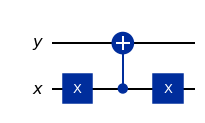
\includegraphics[scale=.5]{images/lab03_1}
\end{figure}
\begin{lstlisting}[style=python]
qx = QuantumRegister(1, 'x')    # input qubit
qy = QuantumRegister(1, 'y')    # output qubit
c  = ClassicalRegister(1, 'c')  # classical bit

circuit = QuantumCircuit(qy, qx, c)
circuit.h(qx)                   # superpose input
circuit.x(qy)                   # prepare output in |1>
circuit.h(qy)                   # superpose output
circuit.barrier()               # separate stages
oracle = deutsch_oracle_circuit()
circuit.compose(oracle, [qy[0], qx[0]], inplace=True)  # apply oracle
circuit.barrier()               # separate stages
circuit.h(qx)                   # interference on input

circuit.measure(qx, c)          # measure input
circuit.draw(output='mpl')      # visualize circuit
\end{lstlisting}
\begin{lstlisting}
random number :  3
\end{lstlisting}
\begin{figure}[h!]\centering
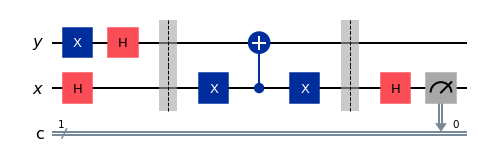
\includegraphics[scale=.5]{images/lab03_2}
\end{figure}
\begin{lstlisting}[style=python]
# simulate circuit with AerSimulator and print counts
from qiskit.transpiler.preset_passmanagers import generate_preset_pass_manager
from qiskit_ibm_runtime import SamplerV2 as Sampler
from qiskit_aer import AerSimulator

aer_sim = AerSimulator()  # create simulator
pm = generate_preset_pass_manager(backend=aer_sim, optimization_level=1) 

isa_circuit = pm.run(circuit)  # transpile circuit
sampler = Sampler(mode=aer_sim)  # create sampler
job = sampler.run([isa_circuit], shots=1)  # run circuit once
result = job.result()  # get results
count = result[0].data.c.get_counts()  # extract counts
print(count)  # print counts
\end{lstlisting}
\begin{lstlisting}
{'1': 1}
\end{lstlisting}
\begin{lstlisting}[style=python]
if ('0' in count) :
	answer = 'constant'
else :
	answer = 'balanced'

print (f'f(x) is a {answer} function.')
\end{lstlisting}
\begin{lstlisting}
f(x) is a balanced function.
\end{lstlisting}

\newpage
\section{Phase Kickback}\label{sec:phase-kickback}

In many quantum algorithms, such as Deutsch, Deutsch--Jozsa, and Bernstein--Vazirani, the \emph{phase kickback} effect allows one to encode information about a Boolean function $f$ into relative phases of a register.  We present here a rigorous derivation and formal statement of phase kickback.

\subsection{Oracle Unitary and Hadamard Eigenstate}
Let $f:\{0,1\}^n\to\{0,1\}$ be a Boolean function, and define the \emph{oracle unitary}
\[
U_f:\mathbb C^{2^n}\otimes\mathbb C^2 \to \mathbb C^{2^n}\otimes\mathbb C^2,
\quad
U_f\bigl(\ket{x}\otimes\ket{y}\bigr)=\ket{x}\otimes\ket{y\oplus f(x)},
\]
where $x\in\{0,1\}^n$, $y\in\{0,1\}$.  As shown in Section~\ref{sec:oracle-def}, $U_f$ is unitary and acts on the second qubit by a conditional bit‐flip.

Define the Hadamard eigenstates on the second qubit:
\[
\ket{+}=H\ket{0}=\tfrac1{\sqrt2}(\ket{0}+\ket{1}),
\qquad
\ket{-}=H\ket{1}=\tfrac1{\sqrt2}(\ket{0}-\ket{1}).
\]

\begin{lemma}[Phase Kickback]
	For any $x\in\{0,1\}^n$, the oracle unitary satisfies
	\[
	U_f\bigl(\ket{x}\otimes\ket{-}\bigr)
	=\ket{x}\otimes X^{f(x)}\ket{-}
	= (-1)^{f(x)}\,\ket{x}\otimes\ket{-}.
	\]
\end{lemma}

\begin{proof}
	Since $X\ket{-}=-\ket{-}$ and $X^0=I$, we have
	\[
	X^{f(x)}\ket{-}
	=\begin{cases}
		\ket{-}, & f(x)=0, \\
		-\ket{-}, & f(x)=1,
	\end{cases}
	= (-1)^{f(x)}\ket{-}.
	\]
	Hence
	\[
	U_f(\ket{x}\otimes\ket{-})
	= \ket{x}\otimes X^{f(x)}\ket{-}
	= (-1)^{f(x)}\ket{x}\otimes\ket{-}.
	\]
\end{proof}

\subsection{Multi‐Qubit Extension}
By linearity, an arbitrary first‐register state $\ket{\psi}=\sum_x a_x\ket{x}$ yields
\[
U_f\bigl(\ket{\psi}\otimes\ket{-}\bigr)
=\sum_{x}a_x(-1)^{f(x)}\ket{x}\otimes\ket{-}
= \bigl(V_f\ket{\psi}\bigr)\otimes\ket{-},
\]
where the \emph{phase oracle} is
\[
V_f=\sum_{x}(-1)^{f(x)}\ket{x}\bra{x}.
\]

\subsection{Applications and Remarks}
\begin{itemize}
	\item In the \emph{Deutsch} algorithm ($n=1$), one starts with $(H\otimes I)U_f(H\otimes H)\ket{0,1}$, and phase kickback yields $(H\otimes I)U_f(\ket{+}\otimes\ket{-})=\pm\ket{0}\otimes\ket{-}$ or $\pm\ket{1}\otimes\ket{-}$, distinguishing constant versus balanced cases with one final Hadamard and measurement.
	\item In \emph{Deutsch--Jozsa} and \emph{Bernstein--Vazirani}, phase kickback on an $n$‑qubit superposition imprints the global phase pattern $(-1)^{f(x)}$, subsequently decoded by an $n$‑fold Hadamard transform.
	\item The phase oracle $V_f$ acts without extra ancilla, showing that any $y$‑qubit initialized to $\ket{-}$ serves as a pure phase marker.
\end{itemize}

This completes the formal lecture notes on phase kickback, a key primitive in quantum algorithmic speed‑ups.
\newpage
\subsection{Exercises}
Consider the two‐qubit unitary evolution \[
\ket{\psi_{\rm in}}
=(H\otimes H)\ket{1,1},
\quad
\ket{\psi'}
=U_f\,\ket{\psi_{\rm in}},
\quad
\ket{\psi_{\rm out}}
=(H\otimes I)\,\ket{\psi'}.
\]
\begin{center}
\begin{quantikz}[column sep=.5cm]
	\lstick{$\ket{1}$} &\gate{H} &\gate[2]{U_f} & \qw &\qw\slice{\scriptsize $\ket{\psi_{\rm out}}$} & \qw &\qw \\
	\lstick{$\ket{1}$} &\gate{H} &             &\gate{H} &\qw & \meter{} &\qw
\end{quantikz}
\end{center}
\begin{enumerate}[(a)]
	\item Show that
	\[
	\ket{\psi_{\rm out}}
	=\frac{1}{2\sqrt2}
	\Bigl[
	(-1)^{f(0)}\ket{00}
	-(-1)^{f(0)}\ket{01}
	+(-1)^{f(1)}\ket{10}
	-(-1)^{f(1)}\ket{11}
	\Bigr],
	\]
	and hence write \(\ket{\psi_{\rm out}}\) as a linear combination of the basis
	\(\{\ket{00},\ket{01},\ket{10},\ket{11}\}\).
	\item Suppose \(f(0)=f(1)=1\).  If the first qubit (\(q_1\)) is measured in the computational basis, compute
	\(\Pr[q_1=1]\) and \(\Pr[q_1=0]\).
\end{enumerate}
\begin{proof}[\normalfont\bfseries\textcolor{magenta}{Sol}]
\textbf{(a)}\; First,
\[
\ket{\psi_{\rm in}}
= (H\otimes H)\ket{1,1}
= \ket{-}\otimes\ket{-}
= \frac1{2}\sum_{x=0}^1\ket{x}\otimes(\ket{0}-\ket{1}).
\]
By phase kickback,
\[
\ket{\psi'}
= U_f(\ket{-}\otimes\ket{-})
= \frac1{2}\sum_{x=0}^1(-1)^{f(x)}\,\ket{x}\otimes(\ket{0}-\ket{1}).
\]
Applying \(H\) on the first qubit gives
\[
\ket{\psi_{\rm out}}
=(H\otimes I)\ket{\psi'}
=\frac1{2}\sum_{x=0}^1(-1)^{f(x)}\bigl(H\ket{x}\bigr)\otimes(\ket{0}-\ket{1})
=\frac{1}{2\sqrt2}\sum_{a,x=0}^1(-1)^{ax+f(x)}\ket{a}\otimes(\ket{0}-\ket{1}),
\]
which is equivalently
\[
\boxed{
	\ket{\psi_{\rm out}}
	=\frac{1}{2\sqrt2}
	\bigl[
	(-1)^{f(0)}\ket{00}
	-(-1)^{f(0)}\ket{01}
	+(-1)^{f(1)}\ket{10}
	-(-1)^{f(1)}\ket{11}
	\bigr].
}
\]

\medskip\noindent\textbf{(b)}\; If \(f(0)=f(1)=1\), then \((-1)^{f(x)}=-1\) for \(x=0,1\).  Substituting,
\[
\ket{\psi_{\rm out}}
=\frac{-1}{2\sqrt2}
\bigl[\ket{00}-\ket{01}+\ket{10}-\ket{11}\bigr]
=\frac{-1}{\sqrt2}\bigl(\ket{00}-\ket{01}\bigr).
\]
Thus the only nonzero amplitudes are on \(\ket{00}\) and \(\ket{01}\), each of magnitude \(1/\sqrt2\).  Consequently,
\[
\Pr[q_1=0]
=\left(-\frac{1}{\sqrt{2}}\right)^2
+\left(-\frac{1}{\sqrt{2}}\right)^2
=\frac12+\frac12=1,
\quad
\Pr[q_1=1]=0.
\]
This completes the solution.
\end{proof}


\newpage
\section{Deutsch--Jozsa Algorithm}
\label{sec:DeutschJozsa}
\subsection{Problem Statement}
Generalize to $f:\{0,1\}^n\to\{0,1\}$ promised either
\begin{itemize}
	\item \emph{constant}: $f(x)$ same for all $x$, or
	\item \emph{balanced}: $f(x)=0$ for exactly $2^{n-1}$ inputs,
\end{itemize}
Classically requires $2^{n-1}+1$ evaluations in worst case; quantum requires one.

\subsection{Algorithm Steps}
\begin{enumerate}
	\item Prepare $n+1$ qubits in $\ket{0}^{\otimes n}\otimes\ket{1}$.
	\item Apply $H^{\otimes(n+1)}$, yielding
	$\ket{\psi_1}=\tfrac1{2^{n/2}}\sum_{x}\ket{x}\otimes\ket{-}$.
	\item Oracle: $\ket{\psi_2}=U_f\ket{\psi_1}=\tfrac1{2^{n/2}}\sum_x(-1)^{f(x)}\ket{x}\otimes\ket{-}$.
	\item Apply $H^{\otimes n}\otimes I$, obtaining
	\[
	\ket{\psi_{out}}=\frac1{2^n}\sum_{y,x}(-1)^{f(x)+x\cdot y}\ket{y}\otimes\ket{-}.
	\]
	\item Measure the first $n$ qubits.
\end{enumerate}

\subsection{Analysis}
The amplitude on $\ket{0^n}$ is \(\displaystyle\frac{1}{2^n}\sum_x(-1)^{f(x)}\),
which equals $\pm1$ if $f$ is constant and $0$ if balanced.  A single measurement thus solves the problem with certainty.

%\subsection{Circuit Diagram}
%\[
%\begin{quantikz}
%	\lstick{\ket{0}^{\otimes n}} & \gate{H}^{\otimes n} & \ctrl{n} & \gate{H}^{\otimes n} & \meter{}\\
%	\lstick{\ket1}               & \gate{H}             & \targ{}  & \qw                   & \qw
%\end{quantikz}
%\]

\newpage
\begin{lstlisting}[style=python]
from qiskit import QuantumCircuit, QuantumRegister, ClassicalRegister  # imports
import numpy as np  # numpy

def dj_oracle_random(n):  # random n-qubit DJ oracle
	qy = QuantumRegister(1, 'y')       # y qubit
	qx = QuantumRegister(n, 'x')       # x qubits
	qc = QuantumCircuit(qy, qx)        # init circuit
	
	np.random.seed()                   # seed RNG
	condition = np.random.choice(['constant', 'balanced'])  # oracle type
	print(condition)                   # debug
	
	if condition == 'constant':        # constant case
		x = np.random.randint(2)       # output bit
		print(x)                       # debug
		# if x==1 f(x)=1, if x==0 f(x)=0
		if x == 1:
			qc.x(qy)                   # flip y
	else:                              # balanced case
		k = np.random.randint(1, n+1)       # number of flips
		a = np.random.permutation(n)        # permute indices
		a = a[:k]                           # take first k indices
		print(a)                            # debug
		for idx in a:
			qc.cx(qx[idx], qy[0])          # CNOT x->y
	
	qc.name = 'D-Jozsa'                # set name
	return qc                          # return oracle

circuit = dj_oracle_random(7)        # build oracle
circuit.draw(output='mpl')           # draw circuit
\end{lstlisting}
\begin{lstlisting}
balanced
[5 2 6 4 1 0 3]
\end{lstlisting}

\begin{figure}[h!]\centering
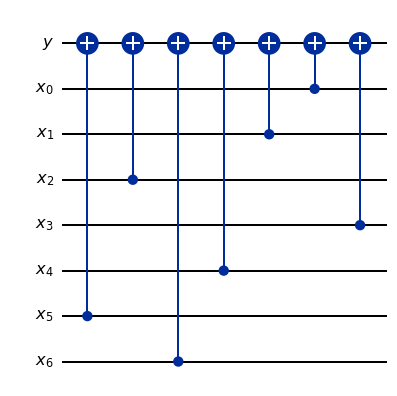
\includegraphics[scale=.5]{images/lab04_1}
\end{figure}

\begin{lstlisting}[style=python]
n = 7
qx = QuantumRegister(n, 'x')                 # input qubits
qy = QuantumRegister(1, 'y')                 # ancilla qubit
c  = ClassicalRegister(n, 'c')               # classical bits
circuit = QuantumCircuit(qy, qx, c)          # init circuit
for qubit in qx:
circuit.h(qubit)                           # H on all x qubits
circuit.x(qy)                                # X on y
circuit.h(qy)                                # H on y
circuit.barrier()                            # barrier
oracle_circuit = dj_oracle_random(n)         # build oracle
circuit.compose(oracle_circuit, qubits=[*qy, *qx], inplace=True)  # apply oracle
circuit.barrier()                            # barrier
for qubit in qx:
	circuit.h(qubit)                           # H on all x qubits
for i in range(n):
	circuit.measure(qx[i], c[i])               # measure x into c
circuit.draw(output='mpl')                   # draw circuit
\end{lstlisting}
\begin{lstlisting}
balanced [0 5 1 4]
\end{lstlisting}

\begin{figure}[h!]\centering
	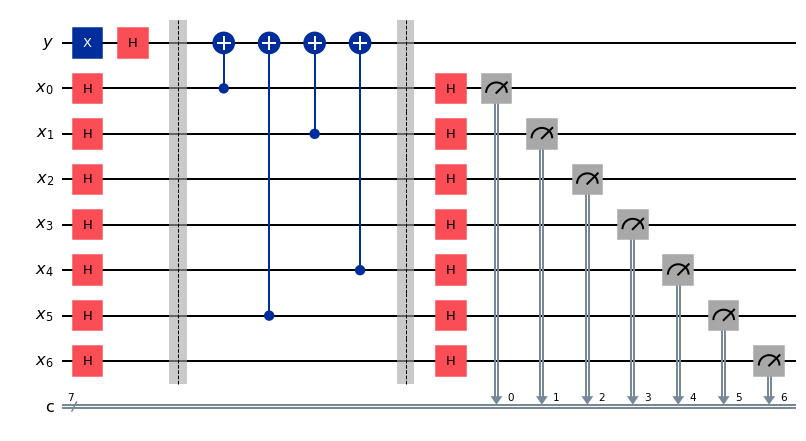
\includegraphics[scale=.5]{images/lab04_2}
\end{figure}

\begin{lstlisting}[style=python]
from qiskit.transpiler.preset_passmanagers import generate_preset_pass_manager
from qiskit_ibm_runtime import SamplerV2 as Sampler
from qiskit_aer import AerSimulator
aer_sim = AerSimulator()
pm = generate_preset_pass_manager(backend=aer_sim, optimization_level=1)
isa_circuit = pm.run(circuit)
sampler = Sampler(mode=aer_sim)
job = sampler.run([isa_circuit], shots=1)
result = job.result()
count = result[0].data.c.get_counts()
print (count)
\end{lstlisting}
\begin{lstlisting}
{'0110011': 1}
\end{lstlisting}

\begin{lstlisting}[style=python]
n_zeros = n*'0'
if (n_zeros in count) : answer = 'constant'
else : answer = 'balanced'
print(f'f(x) is a {answer} function.')
\end{lstlisting}
\begin{lstlisting}
f(x) is a balanced function.
\end{lstlisting}


\newpage
\section{Bernstein--Vazirani Algorithm}
\label{sec:BernsteinVazirani}
\subsection{Problem Statement}
Given oracle access to $f_s(x)=s\cdot x\pmod2$ for unknown $s\in\{0,1\}^n$, determine $s$.  Classically requires $n$ queries; quantum uses one.

\subsection{Algorithm}
\begin{enumerate}
	\item Initialize $\ket{0}^{\otimes n}\otimes\ket1$.
	\item Apply $H^{\otimes(n+1)}$: get $\tfrac1{\sqrt{2^n}}\sum_x\ket{x}\otimes\ket{-}$.
	\item Oracle: $\ket{\psi_2}=\tfrac1{\sqrt{2^n}}\sum_x(-1)^{s\cdot x}\ket{x}\otimes\ket{-}$.
	\item Apply $H^{\otimes n}\otimes I$: by Fourier analysis,
	\[
	(H^{\otimes n}\sum_x(-1)^{s\cdot x}\ket{x})\otimes\ket{-}
	=\ket{s}\otimes\ket{-}.
	\]
	\item Measure first $n$ qubits to read out $s$.
\end{enumerate}

\subsection{Proof of Correctness}
Using $H^{\otimes n}\ket{x}=\tfrac1{2^{n/2}}\sum_y(-1)^{x\cdot y}\ket{y}$, we compute
\[
H^{\otimes n}\Bigl(\sum_x(-1)^{s\cdot x}\ket{x}\Bigr)
=\sum_y\frac1{2^{n/2}}\sum_x(-1)^{s\cdot x + x\cdot y}\ket{y}
=\ket{s},
\]
%as the inner sum vanishes unless $y=s$.  Thus measurement yields $s$ with unit probability citeturn2file4.

\section*{Exercises}
\begin{enumerate}
	\item Prove phase‐kickback more generally: for any $f:\{0,1\}^n\to\{0,1\}$,
	show $U_f(\ket{x}\otimes\ket{-})=(-1)^{f(x)}\ket{x}\otimes\ket{-}$.
	\item Extend Deutsch--Jozsa to detect whether $f$ has Hamming weight $k$.
	\item Analyze robustness of Bernstein--Vazirani against depolarizing noise.
\end{enumerate}

\newpage
\begin{lstlisting}[style=python]
from qiskit import QuantumCircuit, QuantumRegister, ClassicalRegister  # Qiskit imports
import numpy as np  # numpy import

# BV oracle builder
	def bv_oracle_circuit(n, reveal=False):
	qy = QuantumRegister(1, 'y')          # y qubit
	qx = QuantumRegister(n, 'x')          # x qubits
	qc = QuantumCircuit(qy, qx)           # init circuit
	np.random.seed()                      # seed RNG
	s = list(np.random.randint(0, 2, size=n))  # random secret
	if reveal: print("random binary string =", s)  # debug print
	for i in range(n):
		if s[i]:                          # secret bit check
			qc.cx(qx[i], qy[0])          # CNOT x->y
	qc.name = "BV Oracle"                # label circuit
	hs = ''
	for c in reversed(s):
		hs += str(c)                     # build string
	return qc, hs                         # return circuit, secret

circuit, hs = bv_oracle_circuit(5, True)  # build oracle
circuit.draw(output='mpl')               # draw circuit

\end{lstlisting}
\begin{lstlisting}
random binary string =  [1, 1, 1, 0, 1].
\end{lstlisting}

\begin{figure}[h!]\centering
	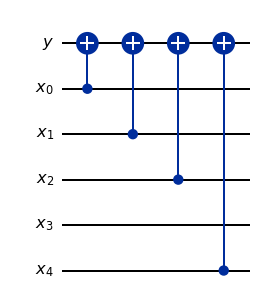
\includegraphics[scale=.5]{images/lab05_1}
\end{figure}

\begin{lstlisting}[style=python]
# build Bernstein-Vazirani circuit
n = 8
qx = QuantumRegister(n, 'x')          # input qubits
qy = QuantumRegister(1, 'y')          # ancilla qubit
c  = ClassicalRegister(n, 'c')        # classical bits
circuit = QuantumCircuit(qy, qx, c)   # init circuit
circuit.h(qx)                         # H on x
circuit.x(qy)                         # X on y
circuit.h(qy)                         # H on y
circuit.barrier()                     # barrier
oracle, hs = bv_oracle_circuit(n, reveal=True)           # build oracle
print(f'hidden string = {hs}')                          # show secret
circuit.compose(oracle, qubits=[qy[0]] + list(qx), inplace=True)  # apply oracle
circuit.barrier()                     # barrier
circuit.h(qx)                         # H on x
circuit.measure(qx, c)                # measure x to c
circuit.draw(output='mpl')            # draw circuit
\end{lstlisting}
\begin{lstlisting}
random binary string =  [1, 1, 0, 1, 1, 0, 1, 1]
hidden string = 11011011
\end{lstlisting}

\begin{figure}[h!]\centering
	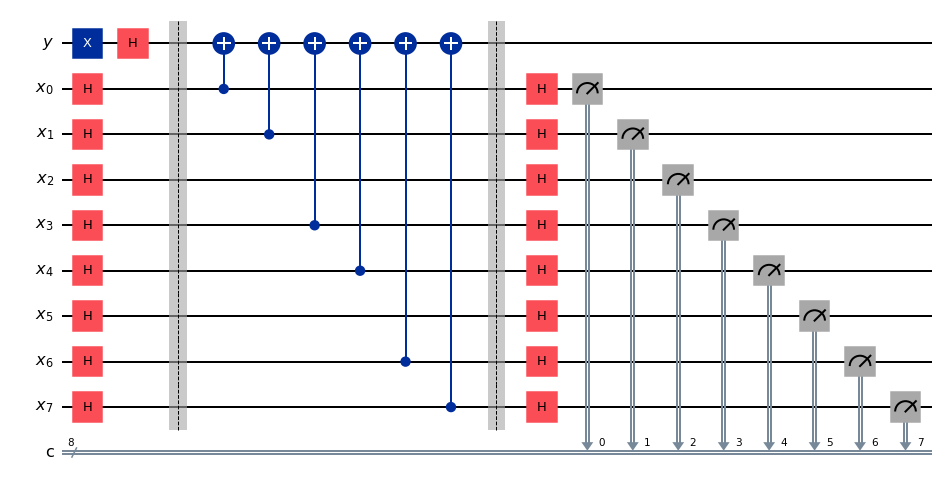
\includegraphics[scale=.5]{images/lab05_2}
\end{figure}

\begin{lstlisting}[style=python]
from qiskit.transpiler.preset_passmanagers import generate_preset_pass_manager
from qiskit_ibm_runtime import SamplerV2 as Sampler
from qiskit_aer import AerSimulator

aer_sim = AerSimulator()
pm = generate_preset_pass_manager(backend=aer_sim, optimization_level=1)

isa_circuit = pm.run(circuit)
sampler = Sampler(mode=aer_sim)
job = sampler.run([isa_circuit], shots=1)
result = job.result()
count = result[0].data.c.get_counts()
print (count)
\end{lstlisting}
\begin{lstlisting}
{'11011011': 1}
\end{lstlisting}

\begin{lstlisting}[style=python]
measured = list(count.keys())[0]

print (f'The measured value {measured} ', end='')
if hs == measured :
	print(f'is equal to the hidden string {hs}')
else :
	print(f'is not equal to the hidden string {hs}')
\end{lstlisting}
\begin{lstlisting}
The measured value 11011011 is equal to the hidden string 11011011
\end{lstlisting}



	
	

	
%%%%%%%%%%%%%%%%%%%%%%%%%%%%%%%%%%%%%%%%%%%%%%%%%%%%%%%%%%%%%%%%%%%%%%
% Appendices
%%%%%%%%%%%%%%%%%%%%%%%%%%%%%%%%%%%%%%%%%%%%%%%%%%%%%%%%%%%%%%%%%%%%%%
\appendix

%\chapter{Appendix A: Additional Build Options}
%For further customization, refer to \texttt{CONFIGURE.md} in the liboqs repository. It details additional build options, including enabling/disabling specific algorithms via the configuration variable \texttt{OQS\_ALGS\_ENABLED}.
%
%\chapter{Appendix B: References}
%\begin{itemize}
%	\item \href{https://github.com/open-quantum-safe/liboqs}{liboqs GitHub Repository}
%	\item \href{https://openquantumsafe.org/}{Open Quantum Safe Project}
%	\item \href{https://github.com/open-quantum-safe/liboqs/blob/main/README.md}{README.md}
%\end{itemize}

\chapter{Exercises}
\section*{Exercises \#1}
\begin{enumerate}[\bfseries 1.]
	\item (Rotation Matrix in the Complex Plane). 
	Let \(\phi\in\mathbb{R}\) and consider the \(2\times2\) matrix  
	\[
	A \;=\;
	\begin{pmatrix}
		\cos\phi & -\sin\phi\\[6pt]
		\sin\phi & \cos\phi
	\end{pmatrix}\!\!.
	\]  
	\begin{enumerate}[(a)]
		\item Prove that \(A\) is a unitary operator on \(\mathbb{C}^2\); that is, show $
		A^\dagger A \;=\; I_2$, where \(A^\dagger\) is the conjugate-transpose of \(A\).
		\item Determine the full spectrum of \(A\) and exhibit for each eigenvalue a corresponding (nonzero) eigenvector.
	\end{enumerate}
\begin{proof}[\normalfont\bfseries\textcolor{magenta}{Sol}] 
\begin{enumerate}[(a)]
	\item Since \(A\) has only real entries, \(A^\dagger = A^T\). Then \begin{align*}
		A^T A
		&=\begin{pmatrix}
			\cos\phi & \sin\phi\\
			-\sin\phi & \cos\phi
		\end{pmatrix}
		\begin{pmatrix}
			\cos\phi & -\sin\phi\\
			\sin\phi & \cos\phi
		\end{pmatrix}\\
		&=\begin{pmatrix}
			\cos^2\phi + \sin^2\phi & -\cos\phi\,\sin\phi + \sin\phi\,\cos\phi\\[6pt]
			-\sin\phi\,\cos\phi + \cos\phi\,\sin\phi & \sin^2\phi + \cos^2\phi
		\end{pmatrix} \\
		&=\begin{pmatrix}
			1 & 0\\
			0 & 1
		\end{pmatrix}.
	\end{align*}
	\item We need to find \(\lambda\in\mathbb C\) and nonzero \(\vec{v}=(v_1,v_2)\) such that $
	A\,\vec{v}=\lambda\,\vec{v}$. Equivalently, \[
	(A-\lambda I_2)\vec{v}=\begin{pmatrix}
		\cos\phi -\lambda & -\sin\phi\\
		\sin\phi & \cos\phi -\lambda
	\end{pmatrix}
	\begin{pmatrix}v_1\\v_2\end{pmatrix}
	=\begin{pmatrix}0\\0\end{pmatrix}.
	\] Nontrivial solutions exist exactly when \[
	\det\bigl(A-\lambda I\bigr)
	=(\cos\phi-\lambda)^2 + \sin^2\phi =0.
	\] Then
	\[
	(\cos\phi-\lambda)^2 + \sin^2\phi
	=\lambda^2 -2\lambda\cos\phi + (\cos^2\phi+\sin^2\phi)
	=\lambda^2 -2\lambda\cos\phi +1,
	\] and so \begin{align*}
	\lambda^2 -2(\cos\phi)\,\lambda +1 =0 &\implies
	\lambda \;=\;\frac{2\cos\phi\pm\sqrt{(2\cos\phi)^2-4\cdot1\cdot1}}{2} \\
	&\implies\lambda=\cos\phi\;\pm\;\sqrt{\cos^2\phi-1}\\
	&\implies\lambda=\cos\phi\;\pm\;\sqrt{-\sin^2\phi}\\
	&\implies\lambda = \cos\phi \pm i\sin\phi
	= e^{\pm i\phi}.
	\end{align*} 
	Thus the two eigenvalues are
	\[
	\lambda_1 = e^{i\phi},\qquad \lambda_2 = e^{-i\phi}.
	\]Since \begin{align*}
		(A-\lambda_1 I)\vec{v}=0
		\implies&\; \begin{pmatrix}
			\cos\phi -(\cos\phi+i\sin\phi) & -\sin\phi\\[6pt]
			\sin\phi & \cos\phi -(\cos\phi+i\sin\phi)
		\end{pmatrix}
		\begin{pmatrix}v_1\\v_2\end{pmatrix}
		=0\\
		\implies&\; \begin{cases}
			(-\,i\sin\phi)\,v_1 \;-\;\sin\phi\,v_2 =0,\\
			\sin\phi\,v_1 \;-\;(i\sin\phi)\,v_2 =0.
		\end{cases}
		\implies\; \begin{cases}
		-iv_1 \;-v_2 =0,\\
	v_1 \;-iv_2 =0.
	\end{cases}\quad\text{if $\sin\phi\neq0$}\\
	\implies&\vec{v}=t\begin{pmatrix}
		1 \\ -i
	\end{pmatrix}\quad\text{with}\; t\neq 0,
	\end{align*}
	a normalized eigenvector is $\displaystyle
	\ket{v_1} = \frac1{\sqrt{2}}\begin{pmatrix}1\\[-3pt]-\,i\end{pmatrix}.$ Similarly, we have $\displaystyle
	\ket{v_2} = \frac1{\sqrt{2}}\begin{pmatrix}1\\[-3pt]i\end{pmatrix}.$
\end{enumerate}
\end{proof}	
	\item (Action of the Kronecker Product on Tensor‐Product Vectors).
	Let  
	\[
	A\in\mathbb{C}^{n\times n},\quad B\in\mathbb{C}^{m\times m},
	\qquad
	\alpha\in\mathbb{C}^n,\quad \beta\in\mathbb{C}^m,
	\]  
	and form their Kronecker products \(A\otimes B\in\mathbb{C}^{(nm)\times(nm)}\) and \(\alpha\otimes\beta\in\mathbb{C}^{nm}\).  Show that  
	\[
	(A\otimes B)\,(\alpha\otimes\beta)
	\;=\;
	(A\,\alpha)\;\otimes\;(B\,\beta).
	\]
\begin{proof}[\normalfont\bfseries\textcolor{magenta}{Sol}]
1. Let \(\{e_i\}_{i=1}^n\) be the standard basis of \(\mathbb{C}^n\) and \(\{f_j\}_{j=1}^m\) the standard basis of \(\mathbb{C}^m\).  By definition of the tensor (Kronecker) product we have the basis  
\[
\{\,e_i\otimes f_j : 1\le i\le n,\;1\le j\le m\}\quad\text{for $\mathbb{C}^n\otimes\mathbb{C}^m\cong\mathbb{C}^{nm}$.}
\] Write
\[
\alpha = \sum_{i=1}^n \alpha_i\,e_i,
\qquad
\beta  = \sum_{j=1}^m \beta_j\,f_j.
\]
Then by bilinearity of the tensor product,
\[
\alpha\otimes\beta
= \sum_{i=1}^n\sum_{j=1}^m 
\bigl(\alpha_i\,\beta_j\bigr)\,(e_i\otimes f_j).
\] By the definition of the Kronecker‐product operator, \[
(A\otimes B)\bigl(e_i\otimes f_j\bigr)
= \bigl(A\,e_i\bigr)\;\otimes\;\bigl(B\,f_j\bigr),
\]
and linearity then gives \[
(A\otimes B)\,(\alpha\otimes\beta)
= \sum_{i=1}^n\sum_{j=1}^m \alpha_i\,\beta_j\,
(A\otimes B)\bigl(e_i\otimes f_j\bigr)
= \sum_{i,j} \alpha_i\,\beta_j\,
\bigl(Ae_i\otimes Bf_j\bigr).
\]
Observe that \[
A\alpha
= A\bigl(\sum_i \alpha_i e_i\bigr)
= \sum_i \alpha_i \,(A\,e_i),
\quad
B\beta
= \sum_j \beta_j \,(B\,f_j).
\]
Hence \[
A\alpha\;\otimes\;B\beta
= \biggl(\sum_i\alpha_i\,Ae_i\biggr)
\otimes
\biggl(\sum_j\beta_j\,Bf_j\biggr)
= \sum_{i,j} \alpha_i\,\beta_j\,
\bigl(Ae_i\otimes Bf_j\bigr)=(A\otimes B)\,(\alpha\otimes\beta).
\]
\end{proof}
	\item % problem 3
	\item % problem 4
	\newpage
	\item (SWAP Gate via Three CNOTs)\;% problem 5
	Let \[
	\mathrm{SWAP}\colon \mathbb{C}^2\otimes\mathbb{C}^2 \to \mathbb{C}^2\otimes\mathbb{C}^2
	\]
	be the two‐qubit operator defined on the computational basis by
	\[
	\mathrm{SWAP}\,\ket{x,y} \;=\; \ket{y,x},
	\quad x,y\in\{0,1\}.
	\]
	\begin{enumerate}[(i)]
		\item Prove that
		\[
		\mathrm{SWAP}
		= \mathrm{CNOT}_{1\to2}\;\circ\;\mathrm{CNOT}_{2\to1}\;\circ\;\mathrm{CNOT}_{1\to2},
		\]
		where $\mathrm{CNOT}_{i\to j}$ denotes a CNOT gate with control qubit $i$ and target qubit $j$.
		\item Show that the following circuit indeed effects the swap of the two qubits:
		\begin{center}
		\begin{quantikz}[column sep=1cm]
			\lstick{$\ket{x}$} & \ctrl{1} & \targ{}    & \ctrl{1} & \qw \\
			\lstick{$\ket{y}$} & \targ{}    & \ctrl{-1} & \targ{}  & \qw
		\end{quantikz}
	\end{center}
	\end{enumerate}
\begin{proof}[\normalfont\bfseries\textcolor{magenta}{Sol}]
	Since both \(U\) and \(\mathrm{SWAP}\) are unitary operators on the two‐qubit Hilbert space, it suffices to check their action on the computational basis \(\{\ket{x,y}:x,y\in\{0,1\}\}\).  Write
	\[
	\mathrm{CNOT}_{1\to2}\,\ket{x,y}
	=\ket{x,\;x\oplus y}, 
	\quad
	\mathrm{CNOT}_{2\to1}\,\ket{a,b}
	=\ket{a\oplus b,\;b},
	\]
	where \(\oplus\) denotes addition modulo~2.	
	
	\medskip
	\noindent\textbf{Step 1:} 
	Apply the first gate:\; $\ket{x,y}
	\;\xmapsto{\;\mathrm{CNOT}_{1\to2}\;}
	\ket{x,\;x\oplus y}.$
	
	\noindent\textbf{Step 2:} Apply the second gate, \(\mathrm{CNOT}_{2\to1}\), to the intermediate state:
	\[
	\ket{x,\;x\oplus y}
	\;\xmapsto{\;\mathrm{CNOT}_{2\to1}\;}
	\ket{\;x\oplus(x\oplus y),\;x\oplus y}
	=\ket{y,\;x\oplus y}.
	\]
	
	\noindent\textbf{Step 3:} Finally apply \(\mathrm{CNOT}_{1\to2}\) again:
	\[
	\ket{y,\;x\oplus y}
	\;\xmapsto{\;\mathrm{CNOT}_{1\to2}\;}
	\ket{y,\;y\oplus(x\oplus y)}
	=\ket{y,\;x}.
	\]
	
	\smallskip
	
	Hence the composite action on an arbitrary basis vector is
	\[
	U\,\ket{x,y}
	=\ket{y,x},
	\]
	which by definition is exactly \(\mathrm{SWAP}\,\ket{x,y}\).
\end{proof}
	\newpage
	\item (Matrix Representation of the Toffoli (CCX) Gate)\;% problem 6
	\begin{center}
		\begin{quantikz}[column sep=1cm]
			\lstick{$q_0$} & \targ{} & \qw\rstick{$q_0\oplus q_1q_2$} \\
			\lstick{$q_1$} & \ctrl{-1} & \qw\rstick{$q_1$} \\
			\lstick{$q_2$} & \ctrl{-1}  & \qw\rstick{$q_2$}
		\end{quantikz}
	\end{center}
	The three‐qubit Toffoli gate (also called the Controlled-Controlled-NOT, or CCX, gate) with qubits \(q_0,q_1\) as controls and \(q_2\) as target acts on the computational basis by
	\[
	\ket{q_0q_1q_2}
	\;\xrightarrow{CCX_{210}}\;
	\ket{(q_0\oplus (q_1\land q_2))q_1q_2},
	\qquad q_0,q_1,q_2\in\{0,1\}.
	\]
	Using the lexicographic ordering
	\(\ket{000},\ket{001},\ket{010},\dots,\ket{111}\),
	represent \(\mathrm{CCX}_{210}\) as an \(8\times8\) unitary matrix.
	
	Let the three-qubit Toffoli gate (also called the Controlled-Controlled-NOT, or CCX, gate) act on the computational basis 
	\(\{\ket{q_0q_1q_2}:q_i\in\{0,1\}\}\) by flipping the target qubit \(q_2\) if and only if both control qubits \(q_0\) and \(q_1\) are in state \(\ket{1}\).  
	
	\begin{enumerate}[(i)]
		\item Write down the action of CCX on each basis vector:
		\[
		\mathrm{CCX}\,\ket{q_0q_1q_2}
		= 
		\ket{q_0\,q_1\,\bigl(q_2 \oplus (q_0\land q_1)\bigr)}.
		\]
		\item Using the standard ordered basis
		\(\ket{000},\ket{001},\ket{010},\ket{011},\ket{100},\ket{101},\ket{110},\ket{111}\),
		represent \(\mathrm{CCX}\) as an \(8\times8\) unitary matrix.
	\end{enumerate}
\begin{proof}[\normalfont\bfseries\textcolor{magenta}{Sol}]
	With the lexicographic ordering
	\(\ket{000},\ket{001},\ket{010},\ket{011},\ket{100},\ket{101},\ket{110},\ket{111}\),
	its matrix representation is the \(8\times8\) unitary
	\[
	\mathrm{CCX}
	=
	\begin{pmatrix}
		1&0&0&0&0&0&0&0\\
		0&1&0&0&0&0&0&0\\
		0&0&1&0&0&0&0&0\\
		0&0&0&1&0&0&0&0\\
		0&0&0&0&1&0&0&0\\
		0&0&0&0&0&1&0&0\\
		0&0&0&0&0&0&0&1\\
		0&0&0&0&0&0&1&0
	\end{pmatrix},
	\]
	i.e.\ the first six basis states are fixed and the last two are swapped.
\end{proof}
\end{enumerate}


\end{document}
